\begin{figure}[htbp]
    \centering
    \definecolor{waterblue}{RGB}{65,190,225}
    \definecolor{waterdark}{RGB}{35,145,190}
    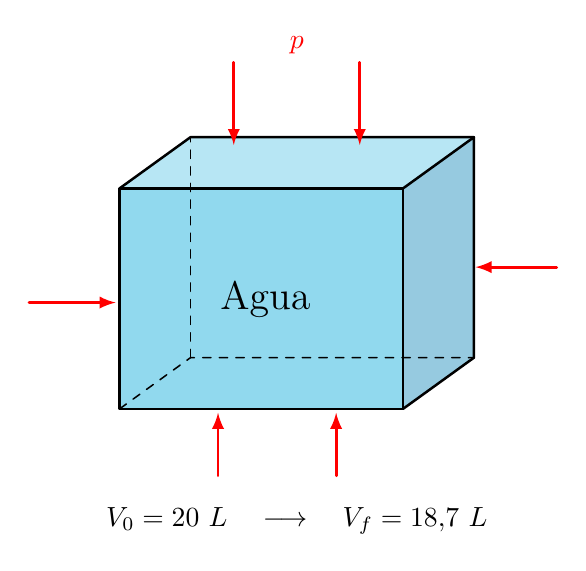
\begin{tikzpicture}[x=1cm,y=1cm,line cap=round,line join=round]
        % Vértices del cubo en perspectiva
        \coordinate (A) at (0,0);
        \coordinate (B) at (3.6,0);
        \coordinate (C) at (3.6,2.8);
        \coordinate (D) at (0,2.8);
        \coordinate (Ap) at (0.9,0.65);
        \coordinate (Bp) at (4.5,0.65);
        \coordinate (Cp) at (4.5,3.45);
        \coordinate (Dp) at (0.9,3.45);

        % Agua dentro del recipiente cúbico
        \fill[waterblue,opacity=0.58] (A) -- (B) -- (C) -- (D) -- cycle;
        \fill[waterdark,opacity=0.48] (B) -- (Bp) -- (Cp) -- (C) -- cycle;
        \fill[waterblue,opacity=0.38] (D) -- (C) -- (Cp) -- (Dp) -- cycle;

        % Aristas visibles del cubo
        \draw[line width=0.9pt] (A) -- (B) -- (C) -- (D) -- cycle;
        \draw[line width=0.9pt] (B) -- (Bp) -- (Cp) -- (C);
        \draw[line width=0.9pt] (D) -- (Dp) -- (Cp);
        \draw[dashed,line width=0.55pt] (A) -- (Ap) -- (Bp);
        \draw[dashed,line width=0.55pt] (Ap) -- (Dp);

        % Etiqueta del fluido
        \node at (1.85,1.38) {\Large Agua};

        % Presión aplicada hacia el interior
        \draw[red,line width=1.0pt,-latex] (1.45,4.40) -- (1.45,3.35);
        \draw[red,line width=1.0pt,-latex] (3.05,4.40) -- (3.05,3.35);
        \draw[red,line width=1.0pt,-latex] (-1.15,1.35) -- (-0.05,1.35);
        \draw[red,line width=1.0pt,-latex] (5.55,1.80) -- (4.52,1.80);
        \draw[red,line width=1.0pt,-latex] (1.25,-0.85) -- (1.25,-0.05);
        \draw[red,line width=1.0pt,-latex] (2.75,-0.85) -- (2.75,-0.05);
        \node[red,above] at (2.25,4.38) {$p$};

        % Cambio de volumen producido por la compresión
        \node[align=center] at (2.25,-1.42)
            {$V_0=20\ \text{L}\quad\longrightarrow\quad V_f=18{,}7\ \text{L}$};
    \end{tikzpicture}
    \caption{Compresión de un volumen cúbico de agua.}
\end{figure}
